\documentclass[letter,10pt,twocolumn,twoside,printwatermark=false]{pinp}

%% Some pieces required from the pandoc template
\providecommand{\tightlist}{%
  \setlength{\itemsep}{0pt}\setlength{\parskip}{0pt}}

% Use the lineno option to display guide line numbers if required.
% Note that the use of elements such as single-column equations
% may affect the guide line number alignment.

\usepackage[T1]{fontenc}
\usepackage[utf8]{inputenc}

% The geometry package layout settings need to be set here...
\geometry{layoutsize={0.95588\paperwidth,0.98864\paperheight},%
          layouthoffset=0.02206\paperwidth,%
		  layoutvoffset=0.00568\paperheight}

\definecolor{pinpblue}{HTML}{185FAF}  % imagecolorpicker on blue for new R logo
\definecolor{pnasbluetext}{RGB}{101,0,0} %


\usepackage{stackengine}

\title{An Introduction to ChemoSpec2D}

\author[a]{Bryan A. Hanson}

  \affil[a]{Dept. of Chemistry \& Biochemistry, DePauw University;
\url{hanson@depauw.edu}}

\setcounter{secnumdepth}{0}

% Please give the surname of the lead author for the running footer
\leadauthor{}

% Keywords are not mandatory, but authors are strongly encouraged to provide them. If provided, please include two to five keywords, separated by the pipe symbol, e.g:
 

\begin{abstract}
A collection of functions for exploratory chemometrics of 2D
spectroscopic data sets such as COSY and HSQC NMR spectra.
\texttt{ChemoSpec2D} deploys methods aimed primarily at classification
of samples and the identification of spectral features which are
important in distinguishing samples from each other. Each 2D spectrum (a
matrix) is treated as the unit of observation, and thus the physical
sample in the spectrometer corresponds to the sample from a statistical
perspective. In addition to chemometric tools, a few tools are provided
for plotting 2D spectra, but these are not intended to replace the
functionality typically available on the spectrometer.
\texttt{ChemoSpec2D} takes many of its cues from \texttt{ChemoSpec} and
tries to create consistent graphical output and to be very user
friendly.
\end{abstract}

\dates{This version was compiled on \today} 

% initially we use doi so keep for backwards compatibility
\doifooter{\url{https://github.com/bryanhanson/ChemoSpec2D}}
% new name is doi_footer

\pinpfootercontents{ChemoSpec2D}

\begin{document}

% Optional adjustment to line up main text (after abstract) of first page with line numbers, when using both lineno and twocolumn options.
% You should only change this length when you've finalised the article contents.
\verticaladjustment{-2pt}

\maketitle
\thispagestyle{firststyle}
\ifthenelse{\boolean{shortarticle}}{\ifthenelse{\boolean{singlecolumn}}{\abscontentformatted}{\abscontent}}{}

% If your first paragraph (i.e. with the \dropcap) contains a list environment (quote, quotation, theorem, definition, enumerate, itemize...), the line after the list may have some extra indentation. If this is the case, add \parshape=0 to the end of the list environment.

\acknow{I'd like to thank Teddy Zartler for encouragement in developing this
package, and for providing valuable test data sets.}

\newcommand\ubar[1]{\stackunder[1.2pt]{$#1$}{\rule{1.2ex}{.075ex}}}

This vignette is based upon \texttt{ChemoSpec2D} version 0.2.19.

\hypertarget{background}{%
\section{Background}\label{background}}

\texttt{ChemoSpec2D} is designed to analyze 2D spectroscopic data such
as COSY and HSQC NMR spectra using appropriate chemometric techniques.
It deploys methods aimed primarily at classification of samples and the
identification of spectral features which are important in
distinguishing samples from each other. \texttt{ChemoSpec2D} stores and
manipulates each spectrum as a matrix of data, and hence a data set is a
collection of 2D spectra. Thus the entire data set is naturally
visualized as a 3D array with dimensions:

\[
\mathrm{F2} \times \mathrm{F1} \times \mathrm{no. \ samples}
\]

or

\[
\mathrm{2D \ Spectrum} \times \mathrm{no. \ samples}
\]

where F2 and F1 are NMR-speak for the x- and y-axes/dimensions. We will
refer to this array as
\(\stackunder[1.2pt]{$\mathbf{X}$}{\rule{1.2ex}{.075ex}}\). See Figure
\ref{3Darray}.

\begin{figure}
\begin{center}
  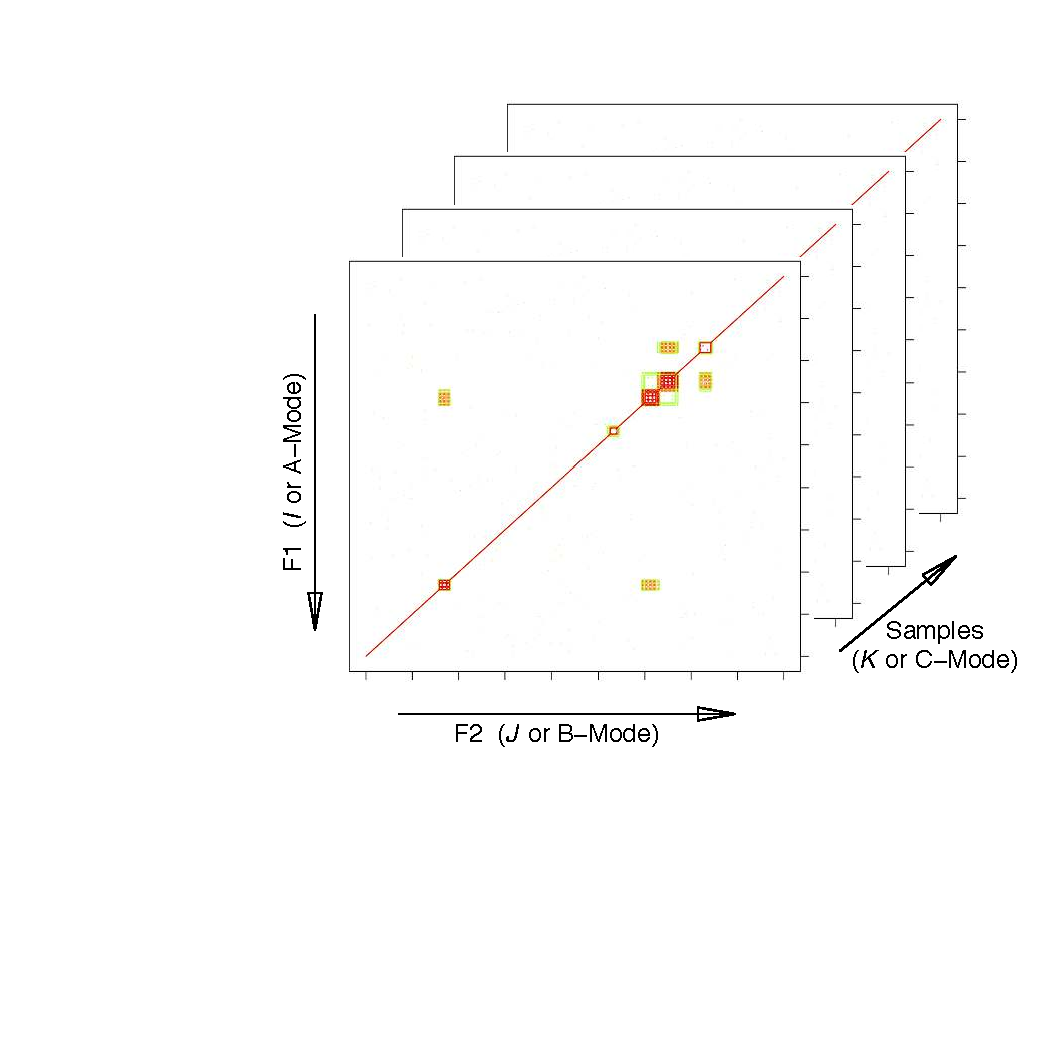
\includegraphics[scale = 0.6]{3Darray.pdf}
  \caption{\label{3Darray}Configuration of data array $\stackunder[1.2pt]{$\mathbf{X}$}{\rule{1.2ex}{.075ex}}$. $I$, $J$ and $K$ are array indices; F2 and F1 are standard terms for NMR dimensions. The mode terminology is typically used in the PARAFAC literature.  This structure is also sometimes referred to as a data cube.}
\end{center}
\end{figure}

\texttt{ChemoSpec2D} treats each spectrum/matrix as the unit of
observation, and thus the physical sample that went into the
spectrometer corresponds to the sample from a statistical perspective.
Keeping this natural unit intact during analysis is referred to as a
\emph{strong} multi-way analysis. In a weak analysis, the 3D data set is
unfolded into a series of contiguous 2D matrices and analyzed using
methods suitable for any 2D data set (such methods are fundamentally
bilinear) (\cite{Huang2003}). In the weak approach, each slice of a 2D
spectrum becomes just another 1D spectrum, and the relationship between
the slices in a single 2D spectrum is lost. Oddly enough, the
trilinear/strong analysis has fewer parameters to estimate so it is
simpler, but computationally more demanding. The interpretation is also
more straight-forward. These techniques are akin to PCA, and seek to
\emph{reduce the data to a limited number components represented by
scores and loadings}. Noise in the data set is reduced, and correlating
variables are collapsed.

The literature on the topics of chemometric analysis of 3D data sets
uses a wide variety of terminology to describe analysis options, and the
same mathematical analysis can be found under different guises in
different fields. Here are some of the more relevant and frequently
encountered terms:

\begin{itemize}
\tightlist
\item
  Multivariate Image Analysis (MIA). This term is typically used when
  the ``images'' are photographs for example, and the term covers a lot
  of ground, such as finding particular objects within a photograph.
  While 2D NMR spectra are typically plotted as contours, there is no
  reason why they cannot be plotted as an image or heat plot, which is
  essentially a photographic image. Classification using MIA methods
  involves a TUCKER1 analysis in which each image is the input, and the
  sample mode (only) is reduced to a requested number of components.
  Scores are the output. \texttt{ChemoSpec2D} can carry out MIA.
\item
  TUCKER3. TUCKER3 is an operation in which all three dimensions of a 3D
  data set are reduced, and each dimension can have a different number
  of components. \texttt{ChemoSpec2D} does not carry out TUCKER3
  analysis.
\item
  PARAFAC. PARAFAC, or parallel factor analysis, is very similar to
  TUCKER3 except that each dimension is reduced to the \emph{same}
  number of components. \texttt{ChemoSpec2D} can carry out PARAFAC and
  it is discussed in greater detail below.
\item
  \(N\)-way Image Analysis. In the case of 2D NMR spectra \(N\) would be
  three. This is a general term term which includes processes such as
  the TUCKER variations and PARAFAC.
\item
  Principal Tensor Analysis (PTA). A tensor is just another term for an
  array of any dimension, so in the case of a collection of 2D NMR the
  data is a 3-way tensor. PTA is not a statistical method, but rather an
  algorithmic option to carry out the statistical computations.
\end{itemize}

Keirs provides discussion and suggestions on terminology best practices
(\cite{Kiers2000}).

\hypertarget{parafac}{%
\section{PARAFAC}\label{parafac}}

\hypertarget{theory-light}{%
\subsection{Theory (Light)}\label{theory-light}}

PARAFAC is ``parallel factor analysis.'' This is a statistical technique
that is somewhat analogous to PCA. Recall that PCA decomposes a 2D data
set into scores and loadings, and is bilinear:

\[
\mathbf{X}^{(n \ \times \ p)} = \mathbf{C}^{(n \ \times \ R)} \times \mathbf{S}^{(R \ \times \ p)} + \mathbf{E}
\]

Where \(\mathbf{X}\) is the raw data, composed of \(n\) samples
\(\times\) \(p\) frequencies, \(\mathbf{C}\) are the scores, and
\(\mathbf{S}\) are the loadings. \(R\) is the number of components
selected. \(R\) is very much smaller than \(p\), as noise and
correlating variables have been reduced. Matrix \(\mathbf{C}\) can be
thought of as ``concentrations'' or weights. Matrix \(\mathbf{S}\) is
composed of ``spectra'' which serve as loadings. \(\mathbf{E}\) consists
of residuals/error. The goal of the PCA algorithm is to solve this
equation and return \(\mathbf{C}\) and \(\mathbf{S}\).

In comparison, PARAFAC decomposes a 3D data set into three matrices, and
is trilinear. Because the data is 3D, standard matrix algebra cannot be
applied. However, the math can be expressed as a summation:

\[
x_{ijk} = \sum_{r = 1}^{R} a_{ir}b_{jr}c_{kr} + \epsilon_{ijk}
\]

Where \(x_{ijk}\) is an element of the 3D data array
\(\stackunder[1.2pt]{$\mathbf{X}$}{\rule{1.2ex}{.075ex}}\). \(a_{ir}\)
is an element of the matrix \(\mathbf{A}\), and so forth for
\(b\)/\(\mathbf{B}\) and \(c\)/\(\mathbf{C}\). \(\epsilon\) is the error
term.

If \(\stackunder[1.2pt]{$\mathbf{X}$}{\rule{1.2ex}{.075ex}}\) is
flattened by taking the \(Kth\)-dimension slices and concatenating them
left-to-right to give a matrix \(\mathbf{X}\), then 2D matrix operations
\emph{can} provide a solution:

\[
\mathbf{X} = \mathbf{A}(\mathbf{C} \odot \mathbf{B})^T + \mathbf{E}
\]

Here, \(\odot\) represents the Khatri-Rao product, a matrix
multiplication variant needed in this situation. \(\mathbf{A}\),
\(\mathbf{B}\) and \(\mathbf{C}\) are the component matrices as above
(\cite{Bro2003b, Smilde2004} Appendix 4.A presents a number of
alternative notations for PARAFAC).

\hypertarget{interpretation}{%
\subsection{Interpretation}\label{interpretation}}

Regardless of the mathematical representation or algorithmic solution,
the results provide \(\mathbf{A}\), \(\mathbf{B}\) and \(\mathbf{C}\).
Interpretation of the component matrices depends upon how
\(\stackunder[1.2pt]{$\mathbf{X}$}{\rule{1.2ex}{.075ex}}\) was
constructed (i.e.~which dimension represents the samples). In the case
of \texttt{ChemoSpec2D} \(\mathbf{C}\) contains values analogous to
scores in that they can be used to see how samples cluster (this is
because the samples are the third dimension of
\(\stackunder[1.2pt]{$\mathbf{X}$}{\rule{1.2ex}{.075ex}}\)). Standard
matrix multiplication of \(\mathbf{A} \ \times \ \mathbf{B^T}\) for a
particular column (component) gives a 2D loading plot (a
pseudo-spectrum) showing the contributions (loadings) of each peak to
the component. \texttt{ChemoSpec2D} uses the \texttt{R} package
\texttt{multiway} to carry out PARAFAC (\cite{Helwig2017}).

PARAFAC is also known by other terms:

\begin{itemize}
\tightlist
\item
  Tensor rank decomposition.
\item
  Canonical polyadic decomposition.
\item
  CANDECOMP (canonical decomposition); PARAFAC and CANDECOMP are the
  same mathematical process but were reported at about the same time and
  given different names by their respective discoverers.
\item
  Tri-linear decomposition.
\end{itemize}

\hypertarget{functions}{%
\section{Functions}\label{functions}}

The list below gives each user-facing function and a brief description
of what it does. Full information is of course available via the help
function, e.g.~\texttt{?sumSpectra2D}. Note that a number of the utility
functions are actually in a supporting package called
\texttt{ChemoSpecUtils} but are loaded automatically when activating
\texttt{ChemoSpec2D}.

\begin{itemize}
\tightlist
\item
  Utility Functions

  \begin{itemize}
  \tightlist
  \item
    \textbf{files2Spectra2DObject} Imports 2D data sets. The format
    options are currently rather limited and not completely vetted!
  \item
    \textbf{chkSpectra} Checks the integrity of a Spectra2D object. This
    can be used directly and is also called by nearly every other
    function to ensure data integrity.
  \item
    \textbf{sumSpectra} Prints a short summary of the Spectra2D object.
  \item
    \textbf{sumGroups} Prints a short summary of the group membership of
    the spectra in a Spectra2D object.
  \item
    \textbf{removeGroup} Remove an entire group from a Spectra2D object.
  \item
    \textbf{removeSample} Remove one or more samples from a Spectra2D
    object.
  \item
    \textbf{removeFreq} Delete selected frequencies (on either
    dimension).
  \item
    \textbf{removePeaks2D} Set selected peaks to NA (on either
    dimension).
  \item
    \textbf{plotSpectra2D} Plots 2D spectra stored in a Spectra2D
    object, as a contour plot. Detailed data exploration is probably
    better done on the spectrometer which is much more suited. This
    function is for quick checks and also publication-quality plots.
  \item
    \textbf{plotSlice} Plots a slice of a 2D spectrum.
  \item
    \textbf{inspectLvls} An easy way to inspect the data in order to
    choose appropriate contour levels.
  \item
    \textbf{normSpectra2D} Normalizes the 2D spectra stored in a
    Spectra2D object.
  \item
    \textbf{centscaleSpectra2D} Centers and scales 2D spectra stored in
    a Spectra2D object.
  \end{itemize}
\item
  Statistical Analysis Functions

  \begin{itemize}
  \tightlist
  \item
    \textbf{pfacSpectra2D} Carries out PARAFAC analysis of the Spectra2D
    object.
  \item
    \textbf{pfacScores} Plots the scores from a PARAFAC analysis. Useful
    for looking at how the samples cluster.
  \item
    \textbf{pfacLoadings} Plots a 2D pseudo-spectrum showing which peaks
    contribute to each component.
  \item
    \textbf{miaSpectra2D} Carries out MIA on a Spectra2D object,
    equivalent to a TUCKER1 analysis.
  \item
    \textbf{miaScores} Plots the scores from MIA.
  \item
    \textbf{miaLoadings} Plots the loadings from MIA.
  \item
    \textbf{plotScree} Plots scree plots from MIA or PARAFAC.
  \end{itemize}
\end{itemize}

\renewcommand{\pnasbreak}{\begin{strip}\vskip0pt\end{strip}}

\phantom{xxx}

%\showmatmethods
\showacknow

\pnasbreak 

\bibliography{ChemoSpec2D}
\bibliographystyle{jss}



\end{document}

